`\section{Methodology}

The proposed study follows a computational approach based on a continuum description of the coupled electromechanical system. 
The methodology is structured in several stages, combining physical modeling with numerical approximation.

First, the governing equations of elasticity and electrical conduction are formulated within a consistent continuum framework. 
The mechanical problem provides the displacement field $u$, from which the strain tensor $\varepsilon(u)$ is computed. 
This strain field serves as input to the electrical problem through the strain-dependent conductivity $\sigma(\varepsilon)$.

As a baseline, the electrical conduction problem with constant conductivity is considered and solved numerically. 
This case admits an analytical solution and is used to validate the numerical implementation. 
A finite element discretization is employed to approximate the solution, and the numerical results are compared against the exact solution.

\begin{figure}[htbp]
    \centering
    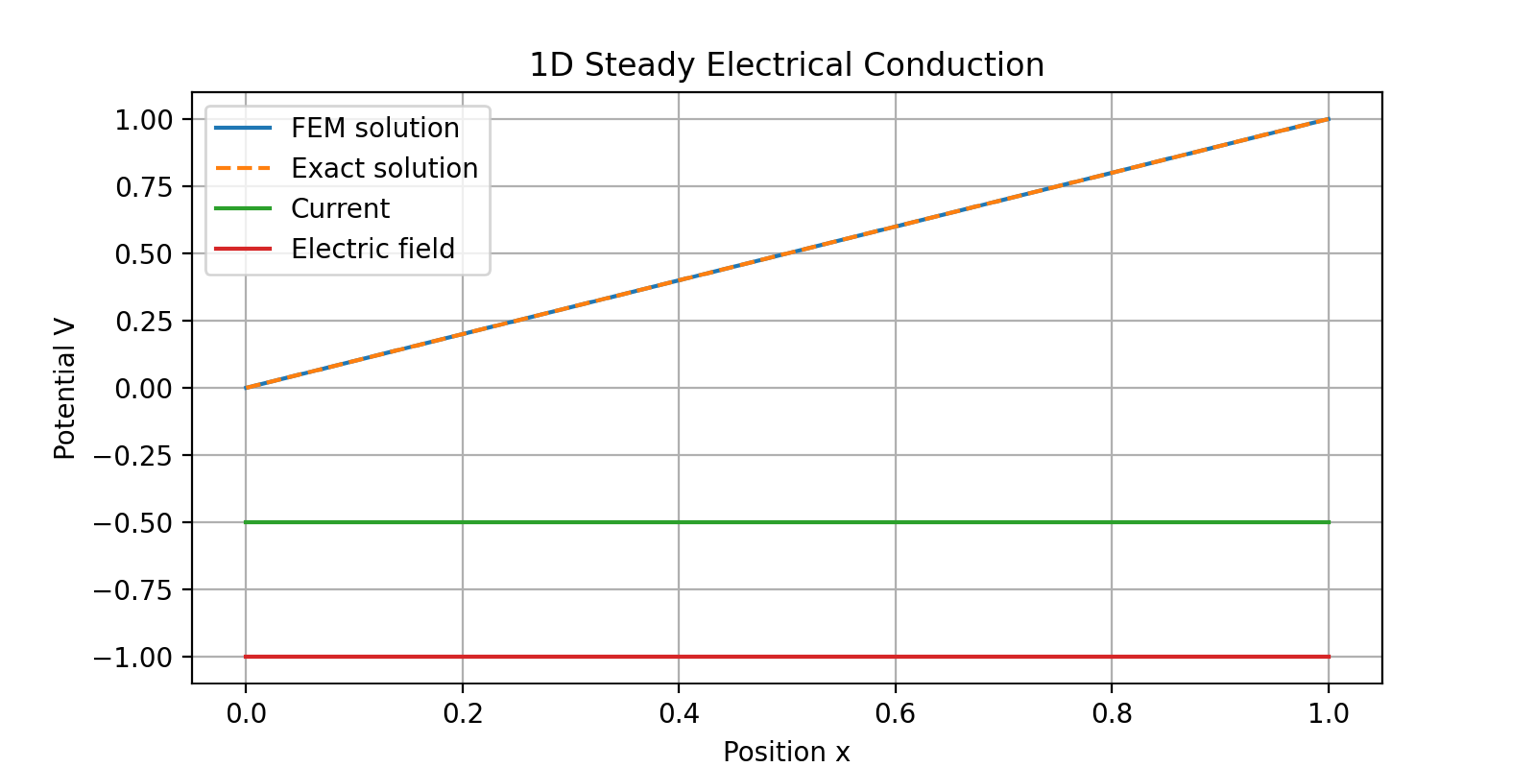
\includegraphics[width=0.75\textwidth]{Images/1d_cond.png}
    \caption{Finite element solution of the 1D steady conduction problem with constant conductivity compared with the analytical solution. 
    The linear potential profile and constant electric field confirm the expected physical behavior.}
\end{figure}

Building on this, the full coupled system is addressed by introducing a spatially varying conductivity $\sigma(\varepsilon(u))$. 
The problem is solved iteratively: the mechanical and electrical fields are updated in a coupled manner until convergence is achieved. 
Special attention is given to the nonlinear nature of the coupling, which may lead to non-uniform fields and sensitivity to deformation.

From a computational perspective, the finite element method (FEM) is used as the primary discretization technique due to its flexibility in handling 
heterogeneous material properties and complex geometries. The implementation focuses on robustness and clarity, enabling systematic exploration 
of different forms of the strain–conductivity relation.

In addition, the methodology allows for extensions beyond purely phenomenological models. 
In particular, the constitutive relation $\sigma(\varepsilon)$ can be treated as a flexible component, 
which may be informed by physical insight or approximated using data-driven approaches. 
This provides a pathway to incorporate more detailed transport behavior without modifying the overall computational framework.

Overall, the methodology is designed to provide a transparent and extensible computational pipeline, 
bridging continuum modeling with physically motivated descriptions of strain-dependent conductivity.'